\chapter{Development of the Kafka Connector Pipeline}
\label{ch04:pipelinedevelopment}

\section{Design and Scope}
The design of the Kafka-based solution is based on a number of goals: ensuring scalability, enabling parallel processing capabilities, and building on the versatility of available Kafka \ac{APIs}. These include the ability to integrate additional components into an existing Kafka pipeline for further processing capabilities or data integration, without requiring extensive time and resources. Furthermore, the solution has to be measurable in terms of performance, both for general monitoring of the system and for comparison to the existing Software GmbH product. Figure \ref{fig:chapter04:overallarchitecture} demonstrates the architecture of the entire replication piper (excluding any additional services for collecting and displaying metrics).

\begin{figure}[htbp]
 \centering
 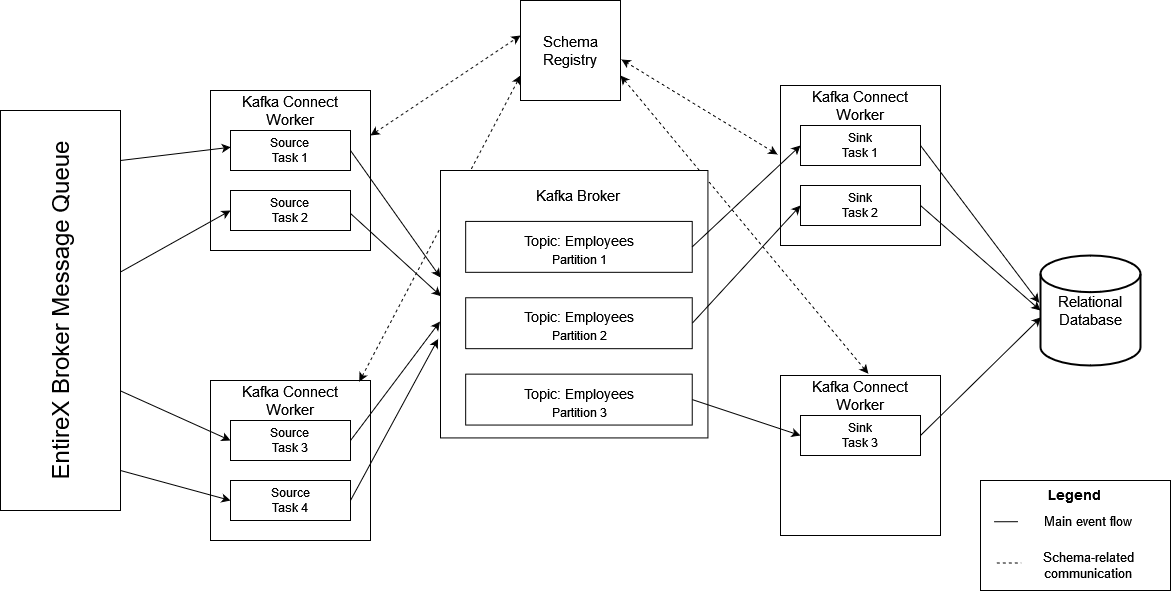
\includegraphics[width=1\textwidth]{chapters/images/kafka pipeline overall architecture enlarged.drawio.png}
 \caption[Overall architecture of Kafka replication pipeline]{Overall architecture of Kafka replication pipeline (see \ref{fig:appendix02:overallarchitecture} for enlarged version)}
 \label{fig:chapter04:overallarchitecture}
\end{figure}

As the solution is intended to be a proof of concept, it is limited in scope. First of all, the solution is currently not intended for full-scale deployment in production. This means that no security measures such as encryption or authorization are supported, and all communication is performed over the \ac{HTTP}. The connectors also lack some functionality due to time constraints, such as no support for replication of coupled files and no support for changes in the \ac{FDT}. Further limitations are discussed in \ref{ch04:pipelinedevelopment:solutionlimitations}.

\section{Implementation Process}
Before the implementation process could properly begin, the design and functionality of Kafka Connect was researched. This involved reading the documentation and looking at available source code of real-life connector implementations. This helped in planning the entire architecture of the solution and the design of the source connector.

\subsection{Implementing the Source Connector}
The main job of the source connector involves consuming any Adabas file change events from the EntireX Broker message queue (see \ref{ch02:fundamentals:adabas:entirex}), transforming the events, and writing them to a specified Kafka topic. There were three main aspects to consider for the connector implementation: how to track changes in the Adabas files, how to divide the work for each task, and how to transform the data to facilitate replication to a relational database further on in the pipeline.
% As explained in \ref{ch02:fundamentals:apachekafkaandkafkaconnect:kafkaconnect}, a connector can run in distributed mode with multiple worker nodes or in standalone mode as a single-process.

\subsubsection{Choosing the Event Replicator as the Source}
There were two strategies being initially considered for tracking Adabas file changes. The first strategy involved adding special \textit{system fields} to the \ac{FDT} that would track the record creation time and the latest change time. The source connector would then be expected to poll the Adabas file at regular intervals and check whether any updates have occurred. This method had major drawbacks, such as the effect that it would have on performance due to regular read commands that would have to be performed. In a production environment where an Adabas file can have over a million records, that can become a major performance bottleneck. This method also fails to identify record deletes. The second strategy, also the one that ended up being implemented, included using the \ac{REPTOR} (see \ref{ch02:fundamentals:adabas:reptor}). Another added advantage of using the \ac{REPTOR} was that the change capture process would be done internally in Adabas, thus minimizing the complexity of the source connector and taking advantage of the mainframe's processing capabilities.

Binary was chosen as the \ac{REPTOR} message format instead of XML due to the performance considerations mentioned in \ref{ch02:fundamentals:adabas:art:limitations}. This required the implementation of a special parser that could interpret the data structures used in the binary format and transform the message into a format that was understood by the connector. The \ac{REPTOR} Parser was implemented to receive an array of bytes representing the message and return the parsed data in the form of a custom DataObject (wrapper class for a HashMap) that contained the message data. The DataObject also contained a custom method for converting the data it contained to a JSON string, adding greater flexibility for further data usage. For a sample binary message and parsed result, see \ref{appendix01:binarymessageexample}.

% \begin{figure}[htbp]
%  \centering
%  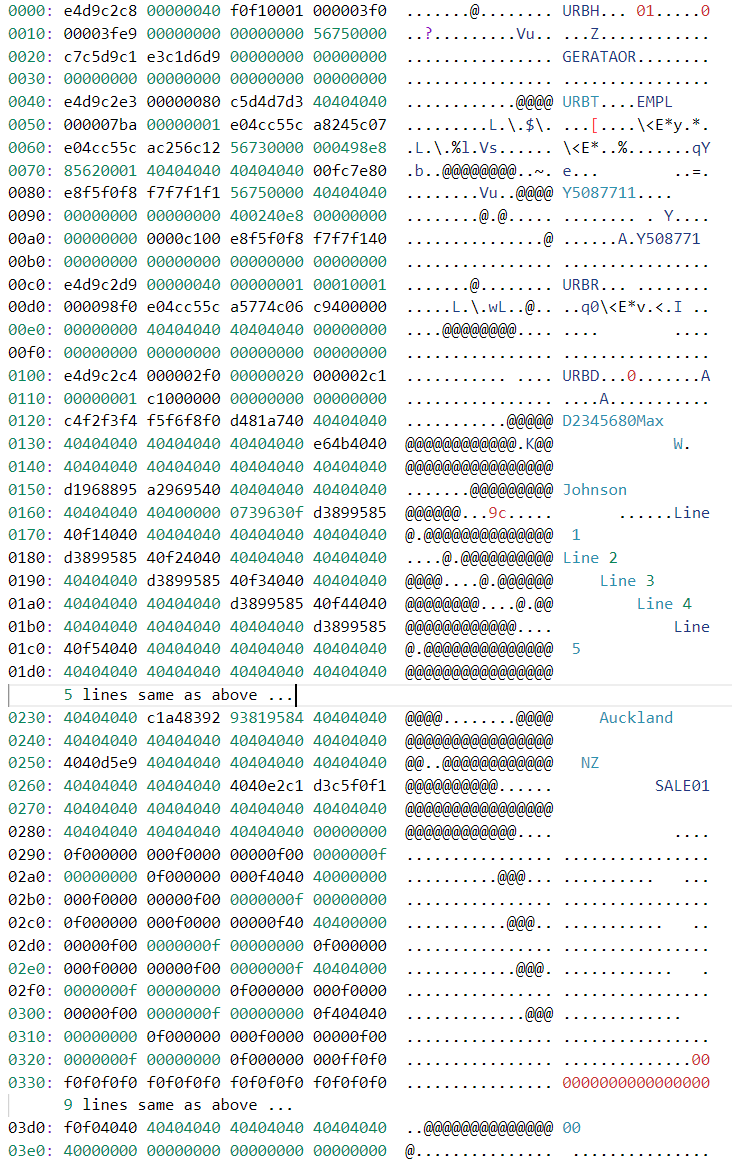
\includegraphics[width=0.49\textwidth]{chapters/images/reptor-parser-binary-light.png}
%  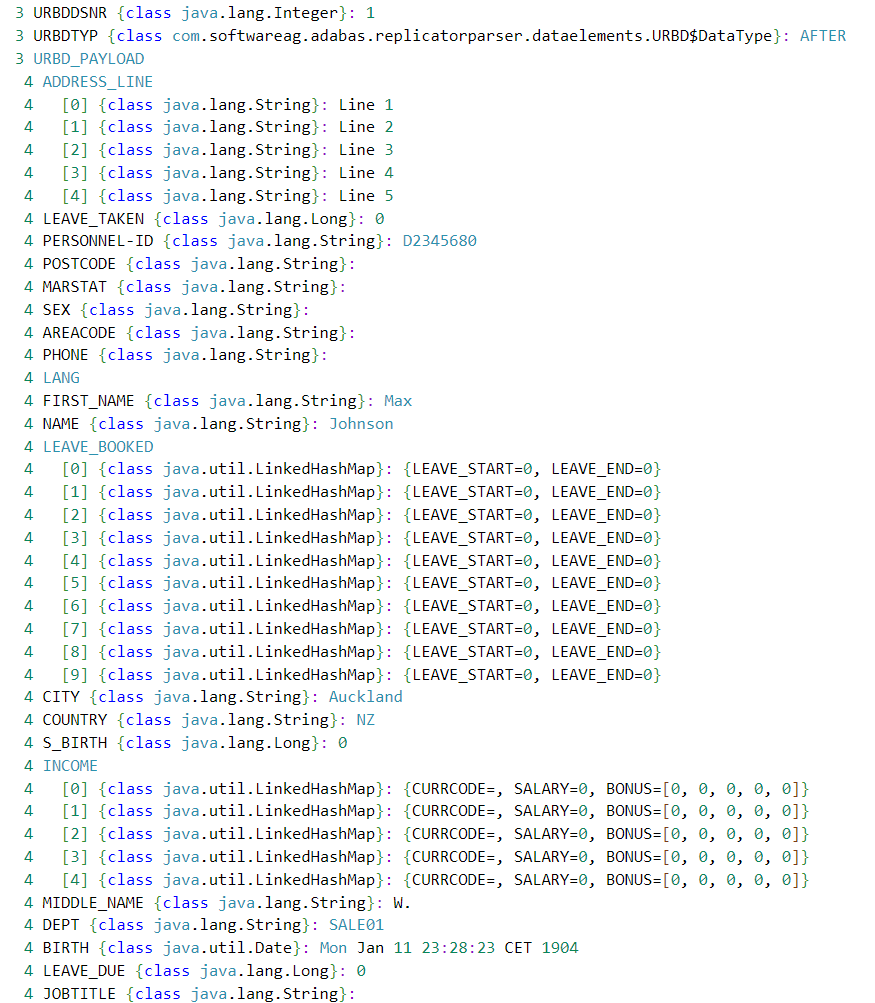
\includegraphics[width=0.49\textwidth]{chapters/images/reptor-parser-parseddataobject-light.png}
%  \caption{Excerpt of a \ac{REPTOR} binary message (left) and the parsed result (right)}
%  \label{fig:chapter04:reptorparserexample}
% \end{figure}
% add to appendix as verbatim

% Figure \ref{fig:chapter04:reptorparserexample} shows the excerpt of a sample binary message and the output of the resulting parsed DataObject. The message in question shows the data image of an Adabas record after an update or insert. Names such as URBDTYP and URBDDSNR represent \ac{REPTOR}-internal data structure fields.

% The second considered strategy included using another Software GmbH product called Adabas Auditing for z/OS. This product also used the EntireX Broker message queue to write auditing events 
% \subsubsection{Writing the Event Replicator Parser} write in upper subsection - to condense

\subsubsection{The Task of Tasks}
To take advantage of Kafka Connect parallelization capabilities, the workload had to be split and distributed to different tasks (the maximum number of tasks is defined in the connector configuration). This is typically done by partitioning the source into different parts and assigning each source partition to one task. However, there was no way to really partition the EntireX Broker message queue. Instead, each task was written to consume from the message queue on a first come first serve basis and process the latest message it received from the queue. Seeing as one \ac{REPTOR} message (or \ac{UOW}) can contain multiple transactions, the task can process multiple events at a time. Each task has an implementation of the \textit{poll} method, which is continuously called and performs the main logic of the task. The polling interval can be specified as a connector configuration.

After the task consumes a \ac{UOW} from the EntireX Broker and parses it with the \ac{REPTOR} Parser, it processes the data and transforms each Adabas record into a number of Kafka records to match the format required for replication to a relational database. The COMMIT message for that specific \ac{UOW} is only sent back to the EntireX Broker after the message has been processed, right before the moment that the Kafka records are returned by the task and written to the Kafka cluster by the connector. Therefore, if the task (or the entire Connect worker) becomes unavailable for any reason while processing a message, the \ac{UOW} will not be marked as processed in the EntireX Broker and can be consumed by another available task in the next poll.
% task processes and only sends commit to broker right before the data is written to kafka 

\subsubsection{Transforming Events to Relational Structure}
\label{ch04:pipelinedevelopment:implementation:transformingtorelational}
To transform an Adabas record to a relational schema, a similar strategy to that of the \ac{ART} default was chosen (see \ref{ch02:fundamentals:adabas:art:schematransformation}). A group field is flattened in the root table, while a new table is generated for each PE group and MU field. However, unlike in the \ac{ART} transformation, no composed index is created of the \ac{ISN} and PE index. Instead, the PE and MU index are set as primary keys additionally to the \ac{ISN} in the respective tables. The root table has the \ac{ISN} as its sole primary key. This was done to enhance table indexing and query performance. Listing \ref{lst:bonusmupequery:connect} shows an example MU field in a PE group generated by the connector, as opposed to the \ac{ART} version shown in Listing \ref{lst:bonusmupequery}. In this case, the primary key fields are the \ac{ISN}, BONUS.IX2, and INCOME.INDEX.

If the schema is auto-generated by the sink connector, no foreign key constraints are created. If foreign key constraints are required, they can either be added manually or the schema can be generated beforehand.
\newpage
\begin{lstlisting}[frame=tb,caption={Query result of the MU field BONUS in the PE field INCOME in the relational table employees\_INCOME\_BONUS (Kafka Connect version)},label=lst:bonusmupequery:connect]
 BONUS | BONUS.IX2 | INCOME.INDEX |  ISN
-------+-----------+--------------+-------
  5000 |         1 |            1 |     1
  2000 |         2 |            1 |     1
  2000 |         3 |            1 |     1
  2500 |         1 |            2 |     1
  2000 |         2 |            2 |     1
\end{lstlisting}
% talk about attempt at using Kafka Streams - leave out for now
% TODO: explain why all messages in one topic

\subsubsection{Writing to Kafka} 
% how were events structured? why all in one topic? how were messages tracked with headers? schema registry?
To write each record to the specified Kafka topic with a message schema, it first has to be constructed as a Kafka Connect-internal "structured record" where the the message structure and content have to be defined, along with a Connect-specific schema definition for that record. The schema is an optional component of Kafka that defines the structure of Kafka messages in a topic. If implemented, the schema can either be sent with every Kafka message, or stored and managed by an additional schema registry. Each schema version has its own ID which also gets stored in each Kafka message, allowing consumers to access the message's specific schema \cite{kafkadatabaseinverted}. This is useful later on for the \ac{JDBC} sink connector, as a way to determine the data types that each field should receive in the target database. The use of schemas is also beneficial in the case that further serialization options, such as Avro, are planned to be added in the future \cite{kreps2011kafka}.

The batch of generated structured records related to the same message are then written to the specified Kafka topic. The message key is set to be the \ac{ISN} of the related Adabas record. Since the default partitioning involves hashing the message key to determine the target partition (see \ref{ch02:fundamentals:apachekafkaandkafkaconnect:apachekafka}), the messages related to the same Adabas record will always end up in the same partition; thus allowing order between the messages for that key to be maintained.
% TODO: add example of message header as verbatim text?

Each Kafka message also contains certain headers which are used to store additional information. One such message header is used for the purpose of determining the table name that each message belongs to\footnote{For instance in the case that the message represents an MU field value.} and the fields that were intended to be primary keys in the target database. Another use for the message header is to track the transaction ID (represented by the transaction commit time), both for tracking the transaction throughput of the sink connector, as well as for identifying which specific transaction the message belongs to. There are other message headers that are generated by the Zipkin service for tracking performance metrics related to each Kafka message (see \ref{ch04:pipelinedevelopment:metrics} for more details). Figure \ref{fig:chapter04:implementation:headerexample} shows a message header containing trace-relevant Zipkin data, as well as the primary key fields and table name. The key can also be seen, showing that this message represents the record with \ac{ISN} 109425.

\begin{figure}[htbp]
 \centering
 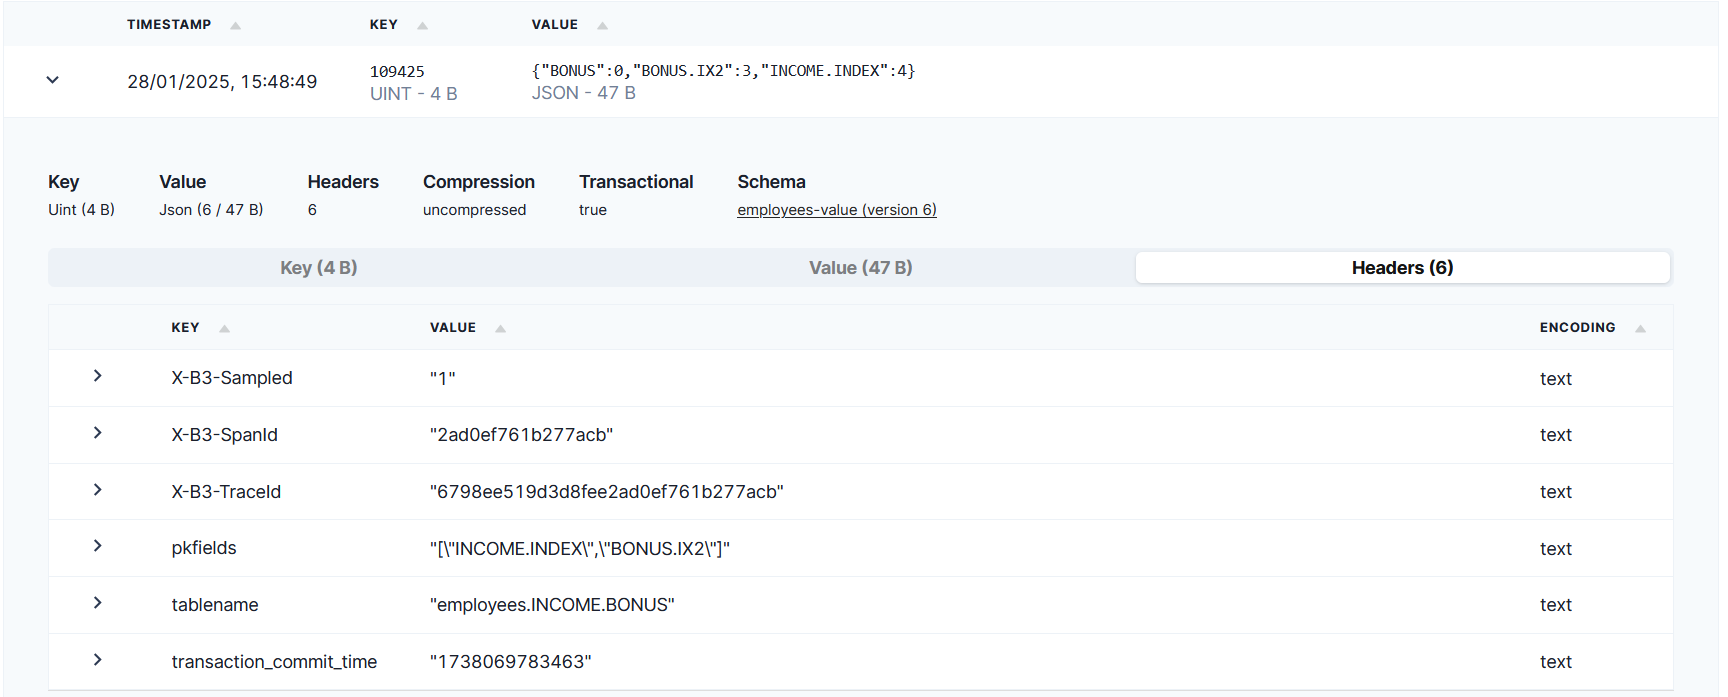
\includegraphics[width=1\textwidth]{chapters/images/header-example.png}
 \caption[Kafka Message with header shown]{Kafka Message with header shown (see \ref{fig:appendix02:implementation:headerexample} for enlarged version)}
 \label{fig:chapter04:implementation:headerexample}
\end{figure}

% TODO: add about transactionality??

\subsection{Implementing the Sink Connector}
Initially, the plan was to implement the \ac{JDBC} sink connector developed by Confluent as it is, without any additional modifications to it. However, some limitations concerning the sink connector cropped up over the course of the implementation, necessitating some modifications to the source code.

\subsubsection{Limitations of Confluent JDBC Sink Connector}
The first limitation encountered by the sink connector was its reliance on topic names to determine the table name in the target database \cite{jdbcsinkdocumentation}. Due to the implementation choice to keep all Kafka records, regardless of the target database table, in the same topic, the sink connector would not have been able to identify the correct target database table name.
% TODO: explain why all messages in one topic further up

Another limitation was the sink connector's inability to set custom primary keys based on the target database table, as is done in \ac{ART}, where MU and PE counters are also treated as primary keys to keep every row identifiable. The available strategies of the sink connector were not meant to handle dynamic primary key definition while allowing the auto-creation of tables and \textit{upserting} of records \cite{jdbcsinkdocumentation}. For more information about the upserting strategy, see \ref{ch04:pipelinedevelopment:parallelizationconsiderations}.

\subsubsection{Modification of Confluent JDBC Sink Connector}
In order to address the sink connector limitations, the source code was pulled and modified. Both the table name and primary key strategy were solved by adding the necessary information to the Kafka message header, providing the sink connector tasks with the necessary information. The source code was then built and Dockerized into a custom image.

\section{Parallelization Considerations}
\label{ch04:pipelinedevelopment:parallelizationconsiderations}
Due to the connectors' distributed nature, aspects such as data consistency and fault tolerance have to be addressed. Due to the source not being partitioned and the tasks in Kafka Connect being designed to run independently of each other, with no way of communicating or synchronizing data, there is guarantee to the order of incoming data and the order that it is written to Kafka by source tasks. For instance, if Task 1 receives a transaction where a record is created, but crashes before processing it, or processes it longer than Task 2 processes a subsequent transaction containing an update on that same record, it is possible that the initial transaction would reach the Kafka broker out of order. This is a challenge generally encountered in distributed systems, where the \ac{CAP} theorem is of great relevance. This theorem states that of the three guarantees listed, only two can be achieved at one time \cite{nookala2022distributedshift}. In the case of our replication solution, an argument can be made that partition tolerance can be theoretically guaranteed between connectors and the Kafka cluster with the configuration of more than one \ac{ISR}. This way, in a scenario where a partition leader node is not reachable, another node can be elected as partition leader \cite{optimizingkafkacap}. Therefore, in line with the theorem, the trade-off can occur either in the availability or the consistency. For this solution, availability was chosen at the cost of strict consistency at the point of the source connector, as afterwards, consistency can be guaranteed by Kafka's offset mechanism. There were two factors that influenced this decision. First of all, if the message order from the source connector proved to be non-negotiable, a further component such as Kafka Streams could be incorporated into the pipeline to handle out-of-order messages before they reach the sink connector \cite{wang2021consistency}. Second of all, in case the order of messages would get mixed up, this wouldn't cause any breaking changes for the sink connector or the target database in the scenario that an update operation of a record would reach the sink connector before the create operation. This is due to the fact that the sink connector has been configured to support \textit{upsert} operations. Thus, if a record is received by the sink connector but does not yet exist in the database, it is inserted instead \cite{jdbcsinkdocumentation}. Furthermore, the \ac{REPTOR} always sends the entire data image of a record, meaning that if a more recent operation reaches the sink connector, the updated state will also contain any changes from previous operations.

% \section{Optimization}
% Some design choices were made in order to optimize the Kafka-based solution.
% not enough for extra section - write about kafka streams in subsection about transforming events to relational structure!

\section{Limitations}
\label{ch04:pipelinedevelopment:solutionlimitations}
% write about transactionality here??
As already demonstrated by the need for custom modifications to the \ac{JDBC} sink connector, there were multiple challenges encountered during the development process. Some of the issues could be resolved with time and effort, while others were too complex to solve in the available time, causing limitations in the scope of this experiment.

The first limitation set is the lack of transactional capabilities of the Kafka solution. While Apache Kafka supports transactionality in the form of "exactly once" delivery guarantees \cite{kafkadocumentation}, not all Kafka Connect components support it. There has been an improvement proposal\footnote{See the Kafka Improvement Proposal 618: \url{https://cwiki.apache.org/confluence/display/KAFKA/KIP-618\%3A+Exactly-Once+Support+for+Source+Connectors}} that adds the "exactly once" delivery guarantee support for source connectors running in distributed mode. However, the \ac{JDBC} sink connector currently only supports the "at least once" delivery guarantee \cite{jdbcsinkdocumentation}. With more time, the \ac{JDBC} sink connector functionality could be extended to provide support for such a delivery guarantee. However, with current available resources, total transaction support had to be left out of the scope. The solution is run with "exactly once" semantics enabled only between the source connector and Kafka brokers.

Another limitation set was the lack of a delete option in the target relational database, as that would have required further development of the custom primary key strategy. The scope was limited only to the create and update operation.

Any changes in the \ac{FDT}, or file schema, were also left out of the scope, as that would require additional tracking and synchronization of any file metadata changes among all the tasks. This can be accomplished in the future with the use of the schema registry service.

Last, but not least, a replication limit of a single Adabas file was set for this scope. While the replication of coupled files could theoretically be accomplished by deploying multiple source connectors (one for each file), this would require further testing.

\section{Metrics}
\label{ch04:pipelinedevelopment:metrics}

\subsection{Monitoring with JMX}
Seeing as Kafka is a Java-based application that runs on the \ac{JVM}, it provides a number of \ac{JMX} metrics with the use of \ac{MBeans}, both for monitoring the system and for basic performance indicators such as broker throughput and latency. Custom metrics can also be added with the \ac{MBeans}, allowing Java applications such as custom connectors to expose metric data relevant to that specific connector. These metrics can then be exposed with the \ac{JMX} exporter agent, allowing them to be collected and evaluated \cite{kafkamonitoringgrafana}. A common stack for monitoring a Kafka-based system involves metric scraping with Prometheus and subsequent visualization (and, if necessary, alerting) with Grafana \cite{applicationmonitoringkafka}.

\begin{figure}[htbp]
 \centering
 \includegraphics[width=1\textwidth]{chapters/images/kafka prometheus monitoring stack enlarged.drawio.png}
 \caption[Monitoring Stack with Prometheus and Grafana]{Monitoring Stack with Prometheus and Grafana (see \ref{fig:appendix02:metrics:prometheusstack} for enlarged version)}
 \label{fig:chapter04:metrics:prometheusstack}
\end{figure}

Figure \ref{fig:chapter04:metrics:prometheusstack} shows an example scenario with two brokers and one Connect worker. Each has a \ac{JMX} exporter running either as part of the application or as a separate Java agent \cite{kafkamonitoringgrafana}. The exporter can be configured to expose certain metrics using a YAML config file, allowing Prometheus to scrape those metrics at regular intervals. Grafana is then used to query the data gathered by Prometheus with the help of \ac{PromQL}, allowing the creation of dashboards for monitoring and data analysis.

% TODO: add screenshot of Grafana dashboard

\subsection{Distributed Tracing}
While \ac{JMX} metrics are useful for monitoring the system as a whole, they typically are not intended for tracing on a per-message basis. Instead, distributed tracing can be implemented with tools such as Zipkin for the tracing of multiple distributed components. In the case of our replication pipeline, a message can be traced with Zipkin from the source connector to the sink connector using the headers in the Kafka message to identify each message. In distributed tracing, a \textit{trace} represents the entire path of the message from the source to the target, while a \textit{span} represents the existence of the message in a specific component of the distributed system \cite{janes2022zipkin}. A trace therefore typically involves multiple spans in a distributed system.

To enable distributed tracing of the Kafka replication solution, an instrumentation library called Brave is used to intercept traces and send them to Zipkin \cite{mallanna2020distributedzipkin}. Such \textit{interceptors} already exist for Kafka Connect in the form of producer and consumer interceptors\footnote{\url{https://github.com/openzipkin-contrib/brave-kafka-interceptor}}. 
Zipkin acts as the collector of the traces and can store them in-memory, or in products with storage and querying capabilities such as Elasticsearch and Cassandra \cite{mallanna2020distributedzipkin}. In this experiment, Elasticsearch was preferred due to existing experience with it. The traces can be indexed and stored in Elasticsearch, then queried and visualized with Kibana. % TODO: add diagram of zipkin

The available interceptors for Kafka Connect allow for the tracing of each produced and consumed Kafka message. To also enable tracing of the entire transaction (which consists of multiple Kafka messages), a custom Zipkin trace was implemented in the source and sink connectors using the Brave library. This allows for the custom metric to measure the throughput transaction of both connectors.


% - JMX good for single components

% - tracing every separate message from start to end, use zipkin

% - measure throughput based on separate records or based on transactions

% Custom JMX metrics in source connector, using existing JMX metrics of all components - some comparable to ART. Using Zipkin for distributed tracing.